\section{Introduction}
\label{sec:introduction}

\begin{figure}[t]
  \centering
  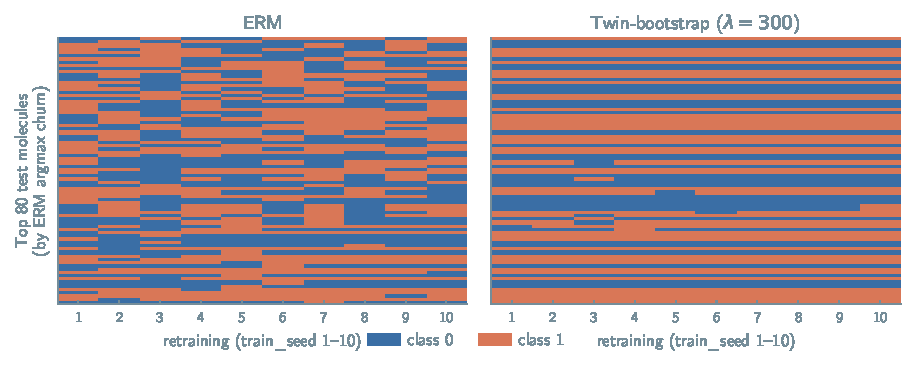
\includegraphics[width=\linewidth]{figures/fig0_overview.pdf}
  \caption{\textbf{Twin-indep eliminates most of ERM's
    retraining-induced prediction flips on BACE.}  Each row is one
    of the $80$ test molecules with the largest cross-sample
    contrast; each column is one of ten retrainings on an
    independent bootstrap of the canonical training pool; cells
    are coloured by predicted class.  Visible vertical stripes
    in the left (ERM) panel are predictions that flip class across
    retrainings; under twin-indep (right; $\lambda{=}300$, matched
    compute against bagging-$K{=}2$) the same molecules become
    near-uniform.  Mean argmax churn over the full test set drops
    from $16.1\%$ (ERM) to $6.4\%$ (twin-indep).}
  \label{fig:overview}
\end{figure}

A toxicity classifier is retrained on a new batch of assay results.
Aggregate accuracy is unchanged.  Predictions flip class for
$8\text{--}17\%$ of candidate molecules, some already in synthesis
queues (Figure~\ref{fig:overview}).  We call this \emph{cross-sample
prediction fragility}: the fraction of test predictions that change
class between two models trained on independent bootstraps of the
same training population.

Equivariant chemistry models bake invariances into the architecture
once --- atom indexing, rotation, conformational degrees of freedom
--- and never re-derive them.  Cross-sample invariance is statistical
rather than architectural, and is the property that determines
whether a deployed prediction survives the next retraining when the
training pool itself changes.

Cross-sample fragility is the population-level analogue of
\emph{prediction churn}~\citep{TODO_milani2016, TODO_bhojanapalli2021,
TODO_jiang2022}.  The deployment-loop literature measures churn
between a new model and a fixed incumbent on web-scale data; we
measure it between two equally weighted bootstraps in the small-$N$
from-scratch regime, where no incumbent exists.  Algorithmic
stability~\citep{TODO_bousquet2002} is the formal anchor.  Deep
ensembles, MC dropout, and conformal prediction all fix the dataset
and vary something else; on our benchmarks they remove
${\sim}2$pp of churn on average.

\paragraph{Contributions.}
\begin{itemize}\itemsep0pt
  \item We re-target prediction-churn measurement to the small-$N$
        from-scratch regime and document its magnitude on eight
        chemistry benchmarks ($8\text{--}17\%$ of predictions flip
        across retrainings; an order of magnitude larger than the
        parameter-variance axis deep ensembles capture).
  \item $K$-bootstrap bagging~\citep{TODO_breiman1996} reduces argmax
        churn $47\text{--}49\%$ on every held-out dataset under a
        no-test-tuning protocol, paired-bootstrap CI excludes zero,
        with no accuracy regression.
  \item Twin-indep is the codistillation
        family~\citep{TODO_anil2018_codistillation} at $\sim$$40\%$
        inter-network bootstrap overlap.  At a frozen
        $\lambda{=}300$ selected on BACE alone, it reduces argmax
        churn $69\text{--}72\%$ at matched compute against
        bagging-$K{=}2$, and distributional disagreement by an
        additional order of magnitude.  On a 10-dataset comparison
        across the overlap axis, $\sim$$40\%$ is the only operating
        point with no failure case (Appendix~\ref{app:overlap_spectrum}).
  \item Per-example fragility computed from a single additional
        bootstrap captures $68\text{--}94\%$ of the test predictions
        that retraining will flip in its top decile.
  \item The methods apply in the small-$N$ from-scratch regime.  On
        pretrained-backbone settings the consistency loss
        over-regularises features the backbone already encodes; on
        datasets where ERM accuracy is close to majority-class,
        consistency methods collapse to the constant predictor.
        Bagging is unaffected by either failure mode.
\end{itemize}

